\subsection{Bluetooth}\label{sec:bluetooth}

\subsubsection{Bluetooth Grundlagen}
Standard-Bluetooth-Geräte senden in einem lizenzfreien Band zwischen 2.402 und 2.480 GHz. Dabei können Störungen durch diverse andere Geräte auftreten, welche im selben Frequenzband arbeiten. Um eine Robustheit gegenüber Störungen zu erhalten, wird ein Frequenzsprungverfahren eingesetzt. Bei diesem Verfahren wird das Frequenzband in 79 Kanäle eingeteilt und bis zu 1600-mal in der Sekunde gewechselt \cite{5_Teildokument_BT}.

Derzeitiger Bluetooth-Standard ist Bluetooth 5. Bluetooth 5 besitzt im Gegensatz zu seinen Vorgängern eine höhere Reichweite (bis zu 100 m statt 25 m) und eine schnellere Datenrate (bis zu 2 Mbit/s statt 1 Mbit/s). Ausserdem enthält dieser Standard ebenso den im Standard 4 bereits eingeführten «Low Energy»-Modus, welcher den schon moderaten Energieverbrauch zusätzlich senkt, was für dieses Projekt benötigt wird \cite{5_Teildokument_BT}. Im Low-Energy-Modus wird für das Frequenzsprungverfahren das Frequenzband nicht in 79- sondern in 40 Kanäle unterteilt. Ausserdem wird auch bei der Datenrate Energie gespart, indem eine Geschwindigkeit von 1- statt 2 Mbit/s erreicht werden kann. Die typische Reichweite im Low-Energy-Modus beträgt 40 m, was die Mindestanforderung von 5 Metern für das Projekt überschreitet und deshalb genügt \cite{6_Teildokument_BT}. Damit über Bluetooth Low Energy (BLE) Verbindungen aufgebaut werden können, benötigt es sogenannte Profile. Bei Bluetooth sind dies das GAP (Generic Access Profile) und das GATT (Generic Attribute Profile). Auf diese wird in den nächsten Kapiteln näher eingegangen.

\subsubsection{Generic Access Profile}
Das GAP kontrolliert Verbindungen und Authentifizierungen. Es beschreibt wie Geräte miteinander kommunizieren. Dazu definiert es zwei verschiedene Rollen für die Geräte. Zum einen die Rolle des zentralen Geräts und zum anderen die Rolle des Peripheriegeräts \cite{7_Teildokument_BT}. Damit eine Verbindung zustande kommt, muss das Peripheriegerät in einem bestimmten Intervall ein Datenpaket das Payload genannt wird, senden. Empfängt ein zentrales Gerät das Payload, kann es für mehr Daten zusätzlich ein Antwortpaket (scan response payload) anfordern, welches daraufhin vom Peripheriegerät gesendet wird \cite{7_Teildokument_BT}. Meistens senden die Peripheriegeräte ihre Authentifizierung, damit eine Verbindung eingegangen und das GATT für mehr Datenaustausch benutzt werden kann. Während diese Verbindung besteht, kann das Peripheriegerät keine weiteren Verbindungen eingehen. Wird jedoch nur eine kleine Datenmenge benutzt, kann diese in das Payload integriert werden, womit alle zentralen Geräte in der Nähe Zugriff auf die Daten haben. Dieses Verfahren nennt man Broadcasting und ist für dieses Projekt von zentraler Bedeutung. Dennoch wird im nächsten Kapitel erläutert, wozu das GATT nützlich ist \cite{7_Teildokument_BT}.

\subsubsection{Generic Attribute Profile}
Das GATT definiert die Art und Weise, wie Peripherie und zentrales Gerät miteinander Daten austauschen. Dies macht es mit Hilfe des Attribute Protocol (ATT) \cite{8_Teildokument_BT}. Das ATT speichert Services, Characteristics und dazugehörende Daten. Services sind logische Sammlungen von zusammengehörenden Characteristics, wobei Characteristics als Datenpunkte angesehen werden können. Demzufolge besteht das ATT aus einer in Services geordneten Datensammlung \cite{8_Teildokument_BT}.

Peripheriegeräte speichern das GATT und dienen somit als GATT-Server. Zentrale Geräte verbinden sich mit Hilfe des GAP mit dem GATT-Server und stellen eine Anfrage. Das zentrale Gerät wird somit zum GATT-Client. In einem Intervall werden vom Client gesendete Anfragen vom Server mit Datenpakete beantwortet. So können grössere Datenpakete ausgetauscht werden, jedoch kein Broadcasting stattfinden \cite{8_Teildokument_BT}. Das genannte zentrale Gerät bzw. GATT-Client ist der Dojo. Die genannten Peripheriegeräte sind BLE-Beacons, welche in der Nähe der Kunstobjekte angebracht sind. Im nächsten Kapitel wird näher auf die BLE-Beacons eingegangen \cite{8_Teildokument_BT}.

\subsubsection{BLE-Beacons}
BLE-Beacons (Bluetooth Low Energy Beacons) sind kleine Peripheriegeräte, welche dazu da sind kleine Informationsmengen zu übertragen. Wird z.B. ein Temperaturverlauf über ein Jahr hinweg gemessen, so kommen BLE-Beacons zum Einsatz, da diese mit einer Knopfzellenbatterie über Jahre hinweg in Betrieb sein können und kleine Informationsmengen übertragen können \cite{9_Teildokument_BT}.

Generell können BLE-Beacons vier Rollen einnehmen. Diese vier Rollen kann man unterteilen in zwei, welche Verbindungen eingehen können, und zwei weitere, welche nicht dazu in der Lage sind. Die Rollen, welche Verbindungen eingehen können, sind zum einen die eines Peripheriegeräts und zum anderen die eines zentralen Geräts. Die, welche keine Verbindungen eingehen können, sind die eines Senders und die eines Beobachters. Als Peripheriegerät fungiert das BLE-Beacon als Slave und wartet somit auf Input des zentralen Geräts (des Masters). Als zentrales Gerät fungiert das BLE-Beacon als Master und kann Verbindungen mit einem oder mehreren anderen Geräten eingehen. Als Sender (Broadcaster) kann das BLE-Beacon zwar keine Verbindngen eingehen, aber z.B. oben erwähnte gemessene Temperatur oder einen vordefinierten Wert senden. Wird das BLE-Beacon als Beobachter (Observer) benutzt, so kann dieser z.B. die von einem anderen BLE-Beacon gesendeten Werte empfangen und an einem angeschlossenen Display anzeigen, jedoch auch keine Verbindungen eingehen \cite{9_Teildokument_BT}. Die übermittelten Signale der BLE-Beacons werden gemäss Abbildung \ref{fig:PacketPayload_Header} formatiert \cite{9_Teildokument_BT}.

\begin{figure}[htbp!!!!]
	\begin{center}
		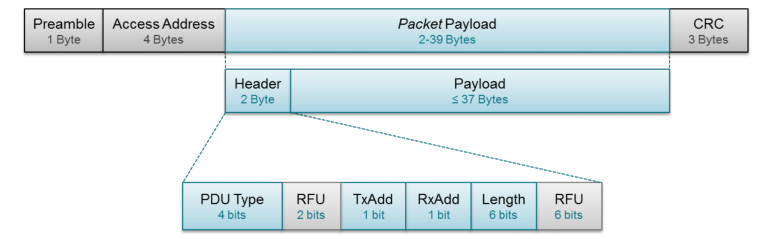
\includegraphics[width=\textwidth]{data/PacketPayload_Header.png}
		\caption[PacketPayload Header]{PacketPayload Header} %picture caption
		\label{fig:PacketPayload_Header}
	\end{center}
\end{figure}

Die Preamble wird zur Synchronisierung und Zeitschätzung benötigt und ist für BLE-Beacons, welche in der Rolle eines Broadcasters sind, immer 0xAA. Auch die Access Address ist für Broadcaster immer gleich, nämlich 0x8E89BED6. Das Packet Payload beinhaltet Header und Payload. PDU bestimmt den Sendekanaltyp des sendenden Beacons, gemäss folgender Tabelle \ref{tab:PDU} \cite{9_Teildokument_BT}:

\begin{table}[htbp!!!]
\begin{tabular}{|c|c|c|}
\hline 
\rule[-1ex]{0pt}{2.5ex} PDU Type & Packet Name & Description \\ 
\hline 
\rule[-1ex]{0pt}{2.5ex} 0000 & ADV{\_}IND & Connectable undirected advertising event \\ 
\hline 
\rule[-1ex]{0pt}{2.5ex} 0010 & ADV{\_}NONCONN{\_}IND & Non-connectable undirected advertising event \\ 
\hline 
\rule[-1ex]{0pt}{2.5ex} 0110 & ADV{\_}SCAN{\_}IND & Scannable undirected advertising event \\ 
\hline 
\end{tabular} 
\caption[PDU Type]{PDU Type}
\label{tab:PDU}
\end{table}

RFU (Reserved for Future Use) steht, wie der Name schon sagt, als Reserve für zukünftige weitere Implementationen und wird deshalb derzeit nicht gebraucht. TxAdd definiert, ob die Sendeadresse des Beacons Öffentlich (TxAdd = 0) oder zufällig (TxAdd = 1) ist. Das RxAdd tangiert Beacons nicht und wird deshalb nicht weiter erwähnt. Das CRC (Cyclic Redundancy Check) dient der Erkennung von Fehlübertragungen. Das Payload ist gemäss Abbildung \ref{fig:PacketPayload_Payload} aufgebaut \cite{9_Teildokument_BT}.

\begin{figure}[htbp!!!!]
	\begin{center}
		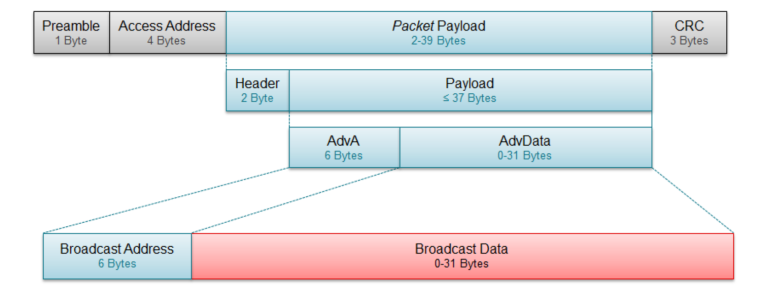
\includegraphics[width=0.8\textwidth]{data/PacketPayload_Payload.png}
		\caption[PacketPayload Payload]{PacketPayload Payload} %picture caption
		\label{fig:PacketPayload_Payload}
	\end{center}
\end{figure}

Es ist zu sehen, dass es mit der Sendeadresse und den Sendedaten gefüllt ist. Die Sendeadresse kann öffentlich oder zufällig sein, wobei eine öffentliche Sendeadresse eine OUI (Organizationally Unique Identifier) nutzt, welche von der IEEE Registration Authority vergeben wird. Die Sendedaten können gemäss der  Tabelle \ref{tab:AD_Data_Type} formatiert werden \cite{9_Teildokument_BT}.

\begin{table}[htbp!!!]
\begin{tabular}{|c|c|c|}
\hline 
\rule[-1ex]{0pt}{2.5ex} AD Data Type & Data Type Value & Description \\ 
\hline 
\rule[-1ex]{0pt}{2.5ex} Flags & 0x01 & Device discovery capabilities \\ 
\hline 
\rule[-1ex]{0pt}{2.5ex} Service UUID & 0x02 - 0x07 & Device GATT services \\ 
\hline 
\rule[-1ex]{0pt}{2.5ex} Local Name & 0x08 - 0x09 & Device name \\ 
\hline 
\rule[-1ex]{0pt}{2.5ex} TX Power Level & 0x0A & Device output power \\ 
\hline 
\rule[-1ex]{0pt}{2.5ex} Manufacturer Specific Data & 0xFF & User defined \\ 
\hline 
\end{tabular} 
\caption[AD Data Type]{AD Data Type}
\label{tab:AD_Data_Type}
\end{table}

Die Flags definieren die Fähigkeiten des BLE-Beacons und sind gemäss der Tabelle \ref{tab:Flags} definiert \cite{9_Teildokument_BT}.

\begin{table}[htbp!!!]
\begin{tabular}{|c|c|c|c|}
\hline 
\rule[-1ex]{0pt}{2.5ex} Byte & Bit & Flag/Value & Description \\ 
\hline 
\rule[-1ex]{0pt}{2.5ex} 0 & • & 0x02 & Length of this data \\ 
\hline 
\rule[-1ex]{0pt}{2.5ex} 1 & • & 0x01 & GAP AD Type Flags \\ 
\hline 
\rule[-1ex]{0pt}{2.5ex} 2 & 0 & LE Limited Discoverable Mode & 180 s advertising \\ 
\hline 
\rule[-1ex]{0pt}{2.5ex} • & 1 & LE General Discoverable Mode & Indefinite advertising time \\ 
\hline 
\rule[-1ex]{0pt}{2.5ex} • & 2 & BR/EDR Not Supported & • \\ 
\hline 
\rule[-1ex]{0pt}{2.5ex} • & 3 & Simultaneous LE and BR/EDR (Controller) & • \\ 
\hline 
\rule[-1ex]{0pt}{2.5ex} • & 4 & Simultaneous LE and BR/EDR (Host) & • \\ 
\hline 
\rule[-1ex]{0pt}{2.5ex} • & 5-7 & • & Reserved \\ 
\hline 
\end{tabular} 
\caption[Flags]{Flags}
\label{tab:Flags}
\end{table}

Die Manufacturer Specific Data können gemäss Tabelle \ref{tab:AD_Data_Type} vom Benutzer definiert werden. Hier können Werte gespeichert werden, die das BLE-Beacon senden soll, wie z.B. den RSSI-Wert. Dieser wird im nächsten Kapitel erläutert \cite{9_Teildokument_BT}.

\subsubsection{RSSI}
RSSI steht für Received Signal Strength Indicator und ist ein Indikator für die Empfangsfeldstärke bei drahtloser Kommunikation. Je höher dieser Wert ist, desto stärker ist das empfangene Signal \cite{10_Teildokument_BT}. Die drahtlose Kommunikation erfolgt über das Senden von elektromagnetischen Wellen. Trifft eine solche Elektromagnetische Welle auf eine Antenne, so führt dies zu einer messbaren Selbstinduktion, welche dem RSSI-Wert entspricht. Dieser Wert muss abhängig von der jeweiligen Anwendung interpretiert werden, da diverse Faktoren bezüglich Transmitter, Receiver und Übertragungsmedium den Wert beeinflussen können.

Im Falle des Museums mit gleichwertigen Beacons bedeutet dies, dass der Besucher sich eher in der Nähe des Beacons mit stärkerem RSSI Wert befindet. Dadurch kann das richtige Audiofile abgespielt werden. Zum Unterscheiden der Beacons werden UUID (Universal Unique Identifier), Major und Minor verwendet. UUID ist im Falle des Projekts eine gewählte Identifikationsnummer für das Museum. Major beschreibt eine eindeutig definierte Zimmernummer und Minor ist die definierte Nummer des Beacons im gleichen Raum. Im nächsten Kapitel wird die Minor- und die Majorvergabe beschrieben.

\subsubsection{Major Minor Vergabe}
Um die Major Minor Nummern mit dem Dōjō zu benutzen, wurden sie im Verlaufe des Projektes standardisiert. Die Sprachauswahl funktioniert über solche Nummern. Beacons mit diesen speziellen Nummern lösen auf dem Dōjō entsprechende Funktionen aus. Abbildung \ref{fig:Bluetooth_def_MM} zeigt die Definitionen. Die Nummernräume sind so gestaltet, dass genug Platz für zusätzliche Funktionen vorhanden ist, wie zum Beispiel für weitere Sprachen oder Zugangskontrollen.

\begin{figure}[htbp!!!!]
	\centering
	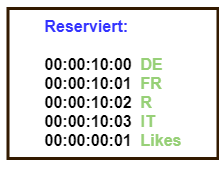
\includegraphics[width=0.3\textwidth]{Data/Reserviert_picture.png}
	\caption[Software:Definierte MM]{Default Definitionen von speziellen Major Minor Nummern.}
	\label{fig:Bluetooth_def_MM}
\end{figure}

In Abbildung \ref{fig:Bluetooth_MM_Vergabe} ist zu sehen, dass die erste Major Nummer 0x00 sein muss, damit ein spezieller Beacon erkennt wird. Das vereinfacht das Programm, da bei einem neuen Ble-Package nur der erste Eintrag im Array betrachtet werden muss, um die speziellen Beacons zu erkennen. Der Nummernraum für spezielle Beacons umfasst ca 16 Mio. Adressen, was für zusätzliche Funktionen reichen sollte. Sommit bleiben ca 4.2 Mia. Adressen für Kunstwerke übrig.

\begin{figure}[htbp!!!!]
	\centering
	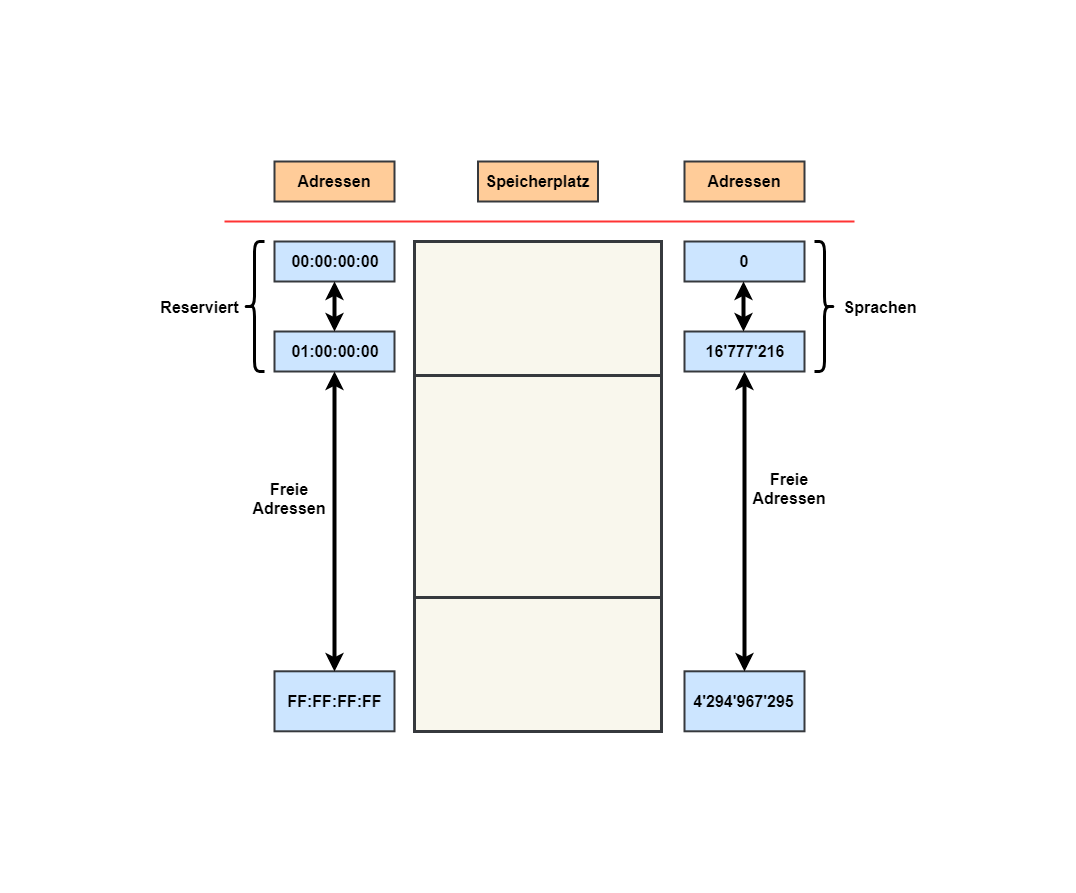
\includegraphics[width=0.9\textwidth]{Data/Speicheradressen_picture.png}
	\caption[Software:MM Vergabe]{Definition der Majo Minor Vergabe}
	\label{fig:Bluetooth_MM_Vergabe}
\end{figure}



